\documentclass{article}
\usepackage[margin=1in]{geometry}
\usepackage{amsmath}
\usepackage{amssymb}
\usepackage{graphicx}
\usepackage{float}

\title{Report for Programming Assignment 1}
\author{Vishwak Srinivasan\\
\texttt{CS15BTECH11043}}
\date{}

\begin{document}
\maketitle
\begin{flushleft}
The ``special" functions in consideration for this assignment were:
\begin{gather*}
f_{Q}(x, y) = 1.125x^2 + 0.5xy + 0.75y^2 + 2x + 2y \\
f_{LL}(x, y) = 0.5(x^2 + y^2) + 50\log\left(1 + e^{-0.5y}\right) + 50\log\left(1 + e^{0.2x}\right) \\
f_{H}(x, y) = 0.1(x^2 + y - 11)^2 + 0.1(x + y^2 - 7)^2 \\
f_{R}(x, y) = 0.002(1 - x)^2 + 0.2(y - x^2)^2
\end{gather*}

These functions were plotted using \texttt{GNUplot}, a terminal based plotting tool. The code for plotting can be found in the file: \texttt{plotter.gnuplot}. A few important observations could be made:
\begin{itemize}
\item In the domain of consideration i.e., \([-6, 6]\times[-6, 6]\) for \(f_{Q}, f_{LL} \text{ \& } f_{H}\) and \([-3, 3] \times [-6, 6]\) for \(f_{R}\) --- \(f_{Q}\) and \(f_{LL}\) were found to convex, and \(f_{H}\) and \(f_{R}\) were found to be non-convex. All these inferences were based of the surfaces plotted.
\item \(f_{Q}\) and \(f_{LL}\) have 1 minimum each, whereas \(f_{H}\) has 4 local minima and 1 local maximum. The problem with \(f_{R}\) is the existence of a valley like structure.
\end{itemize}

\begin{figure}[H]
\begin{minipage}{0.45\linewidth}
\centering
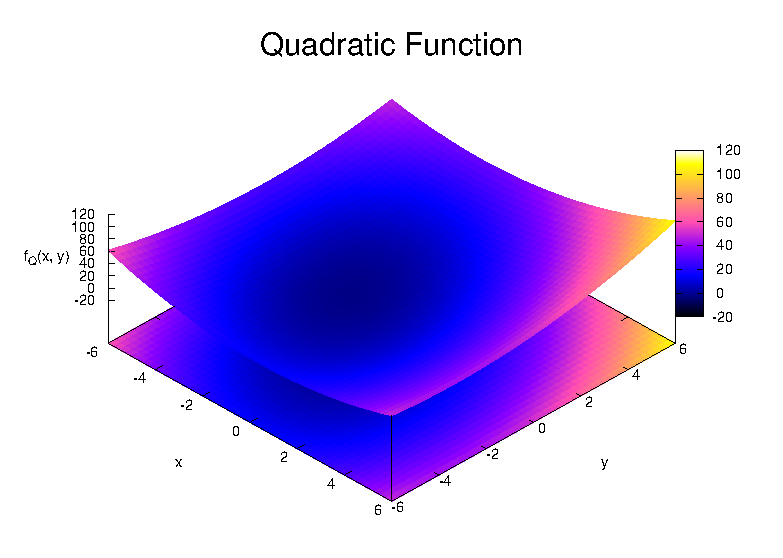
\includegraphics[width=0.75\textwidth]{quadratic_function}
\caption{Note the basin (dark region in the middle)}
\end{minipage}
\hfill
\begin{minipage}{0.45\linewidth}
\centering
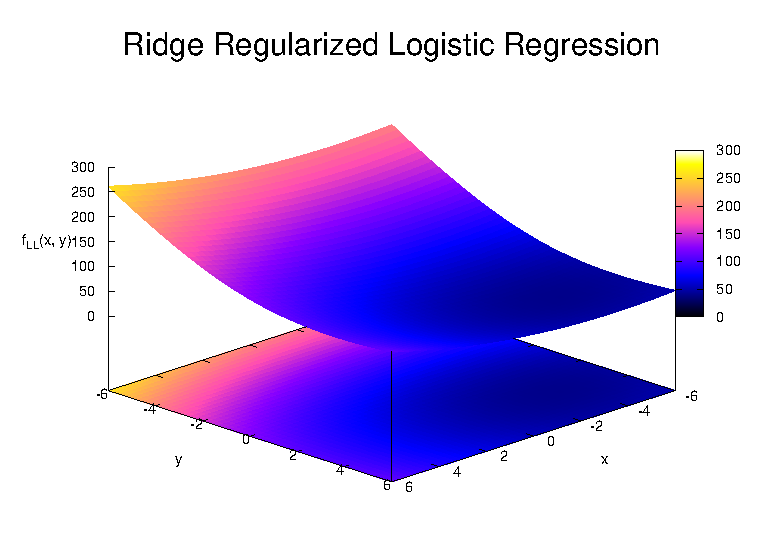
\includegraphics[width=0.75\textwidth]{ridge_regularized_logistic_regression}
\caption{Note the basin (slightly darker region near \((-4, 4)\))}
\end{minipage}
\end{figure}

\begin{figure}[H]
\begin{minipage}{0.45\linewidth}
\centering
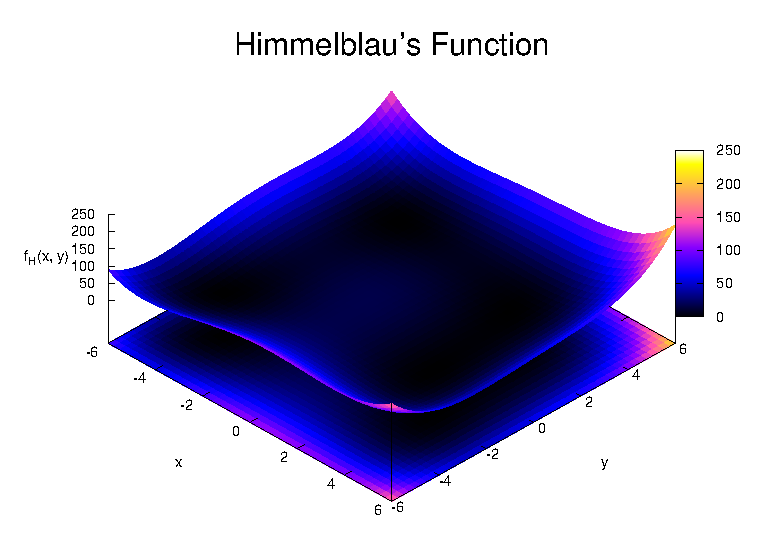
\includegraphics[width=0.75\textwidth]{himmelblaus_function}
\caption{Note the 4 basins and a plateau approximately in the middle of them}
\end{minipage}
\hfill
\begin{minipage}{0.45\linewidth}
\centering
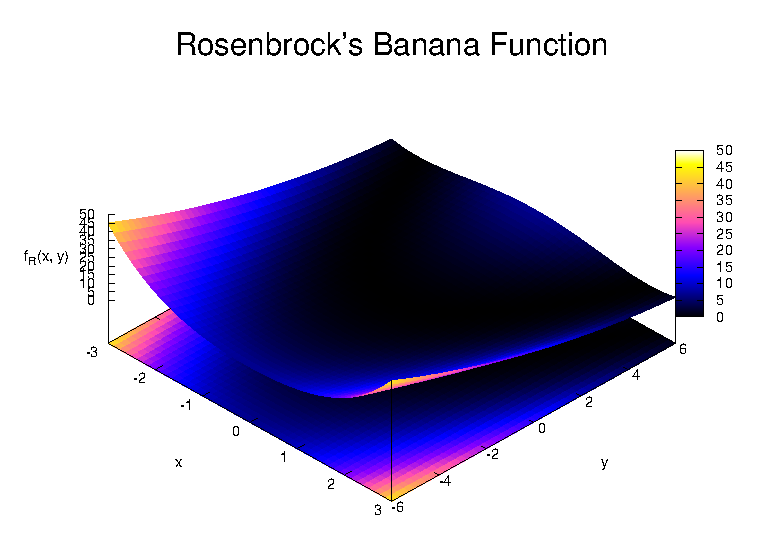
\includegraphics[width=0.75\textwidth]{rosenbrock_banana_function}
\caption{Note the valley (dark parabolic structure)}
\end{minipage}
\end{figure}

Gradient Descent was the algorithm used to find attain the closest minimum from the point of initialization. The reason \textit{closest minimum} is explicitly mentioned is because of the existence of multiple minima in the Himmelblaus function, and the dynamics of Gradient Descent dictate that the result of the algorithm will lie at the closest basin of attraction.
\(\newline\)

The first Gradient Descent method used was Vanilla Gradient Descent with a fixed step size to be chosen from \(\lbrace 0.3, 0.1, 0.01 \rbrace\). The point of initializations were one fixed point -- \((2,3)\) for all functions and two other points chosen randomly from the domain in consideration of the functions. My implementation chooses these points from a uniform distribution over the domain of the functions.
\(\newline\)

We are going to evaluate the performance of different learning rate settings for the static initialization at \((2,3)\) by considering the different in the function values at the optimal and last update i.e., \(1000^{th}\) iteration. The optimal values calculated analytically (or using the Newton-Raphson method for \(f_{LL}(x, y)\)) are as follows:
\begin{center}
\begin{tabular}{|c|c|c|}
\hline
Function & Optimal Value in domain & Attained at \\
\hline
Quadratic Function & \(0.0\) & \((-0.64, -1.12)\)\\
\hline
Ridge Regularized Logistic Regression & \(\approx 40.4012\) & \((-3.3742, 3.5787)\)\\
\hline 
Himmelblaus Function & \(0.0\) & \((3, 2)\)\\
\hline
Rosenbrock's Banana Function & \(0.0\) & \((1, 1)\)\\
\hline
\end{tabular}
\end{center}

\begin{center}
\begin{tabular}{|c|c|c|c|}
\hline
& 0.3 & 0.1 & 0.01 \\
\hline
\(f_{Q}(x, y)\) & & & \\
\hline
\(f_{LL}(x, y)\) & & & \\
\hline
\(f_{H}(x, y)\) & & & \\
\hline
\(f_{R}(x, y)\) & & & \\
\hline
\end{tabular}
\end{center}

\end{flushleft}
\end{document}
